\documentclass[12pt,a4paper]{report}
\usepackage[english]{babel}
\usepackage[utf8]{inputenc}
\usepackage{color}
\usepackage{amsmath}
\usepackage{mathtools}
\usepackage{graphicx}
\usepackage[export]{adjustbox}
\usepackage{subcaption} %per le figure doppie 
\usepackage{array}
\usepackage{multirow}
\usepackage{tabularborder}
\usepackage{footnote}
\usepackage{caption}
\usepackage{siunitx}
\usepackage{hyperref}
\usepackage{newlfont}
\usepackage{color}
\usepackage{url}
\textwidth=450pt\oddsidemargin=0pt
\usepackage{hyperref}
\usepackage{fancyhdr}
\pagestyle{fancy}
\usepackage[Lenny]{fncychap}


\begin{document}




\setlength{\headheight}{15pt}



\begin{titlepage}
%
%
% ONCE YOU ARE FINISHED WITH YOUR CHANGES MODIFY "RED" WITH "BLACK" IN ALL \textcolor COMMENTS
%
%
\begin{center}
{{\Large{\textsc{Alma Mater Studiorum $\cdot$ University of  Bologna}}}} 
\rule[0.1cm]{15.8cm}{0.1mm}
\rule[0.5cm]{15.8cm}{0.6mm}
\\\vspace{3mm}
{\small{\bf School of Science \\
Department of Physics and Astronomy\\
Master Degree in Physics}}
\end{center}

\vspace{23mm}

\begin{center}\textcolor{black}{
%
% INSERT THE TITLE OF YOUR THESIS
%
{\Large{\bf Implementation of an automated pipeline for predicting the response to neo-adjuvant chemo-rediotherapy of colorectal cancer}}
}\end{center}

\vspace{50mm} \par \noindent

\begin{minipage}[t]{0.47\textwidth}
%
% INSERT THE NAME OF THE SUPERVISOR WITH ITS TITLE (DR. OR PROF.)
%
{\large{\bf Supervisor: \vspace{2mm}\\\textcolor{black}{
Prof. Gastone Castellani}\\\\
%
% INSERT THE NAME OF THE CO-SUPERVISOR WITH ITS TITLE (DR. OR PROF.)
%
% IF THERE ARE NO CO-SUPERVISORS REMOVE THE FOLLOWING 5 LINES
%
\textcolor{black}{
\bf Co-supervisor: \vspace{2mm}\\Dr. Nico Curti\\\\}}}
\end{minipage}
%
\hfill
%
\begin{minipage}[t]{0.47\textwidth}\raggedleft \textcolor{black}{
{\large{\bf Submitted by:
\vspace{2mm}\\
%
% INSERT THE NAME OF THE GRADUAND
%
\textcolor{black}{
Giuseppe Filitto}}}
}
\end{minipage}

\vspace{32mm}

\begin{center}
%
% INSERT THE ACADEMIC YEAR
%
Academic Year \textcolor{black}{ 2020/2021}
\end{center}

\end{titlepage}


\clearpage

\begin{abstract}
    Colorectal cancer is a malignant neoplasm of the large intestine resulting from the uncontrolled proliferation of the cells making up the colorectal tract.
    Colorectal cancer isthe second malignant tumor per number of deaths after the lung cancer and the thirdfor number of new cases after the breast and lung cancer. Risk factors for this kind of cancer include colon polyps, long-standing ulcerative colitis, diabetes of type II and also genetic history (HNPCC or Lynch syndrome). In order to get information about diagnosis, therapeutic effect evaluation on colorectal cancer, radiomic analysis can be performed on radiological images through the application of dedicated radiomic algorithms based on segmentation and features extraction. By segmentation we mean the determination of the regions of interest (ROI) in images that are going to be analyzed. In clinical routines, it is carried with manual or semi-manual techniques by radiologists, but this process is time-consuming, highly operator-dependent and subject to operator expertise. By Radiomic features we meant the features coming from radiographic medical images, which can potentially uncover disease characteristics that fail to be appreciated by the naked eye.
    The aim of this project is to implement an automated pipeline based on automatic segmentation of T2 weighted Magnetic Resonance (MR) images exploiting Convolutional Neural Networks in order to predict the response to neo-adjuvant chemo-radiotherapy of colorectal cancer using radiomics features.
\end{abstract}

\clearpage
\thispagestyle{empty}
\begin{flushright}
\null\vspace{\stretch{1}}
\large{\emph{\dots To my family and Nicole}}
\vspace{\stretch{2}}\null
\end{flushright}


\clearpage
\tableofcontents


\chapter{Introduction}

Colorectal cancer is a malignant neoplasm of the large intestine resulting from the uncontrolled proliferation of the cells making up the colorectal tract.
Colorectal cancer is the second malignant tumor per number of deaths after the lung cancer and the third for number of new cases after the breast and lung cancer\cite{cancerstats}.
Among the risk factors for this kind of cancer non hereditary could range from colon polyps to long-standing ulcerative colitis, from Crohn's disease to old age. Also genetic history (HNPCC or Lynch syndrome) and nutritional factors as
diabetes II can increase the probability of develop cancer \cite{tesicoppola}.
Preventive measures for colorectal cancer include physical activity, reducing the consumption of processed meat and alcohol, and avoiding smoking\cite{stats2019}.

\begin{figure}[h!]
	\centering
	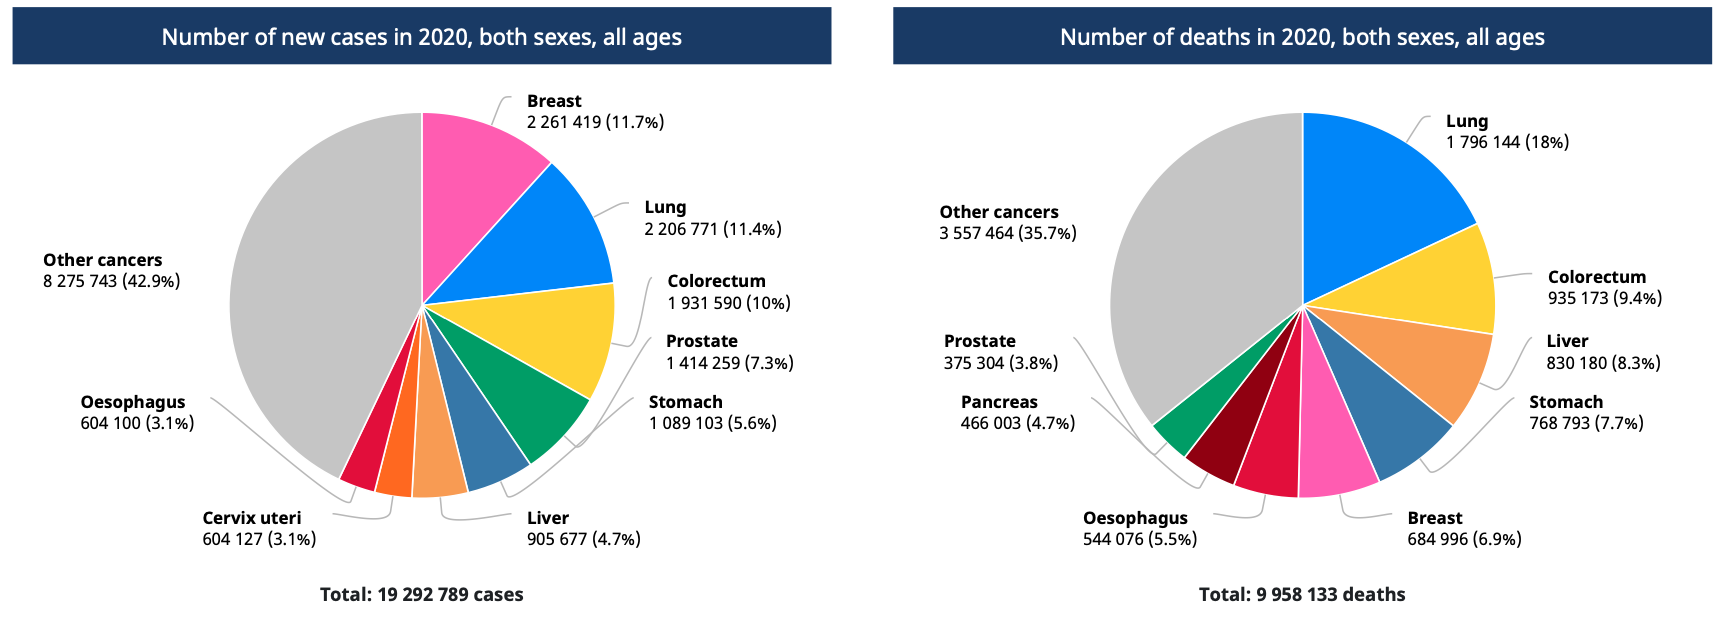
\includegraphics[width=0.8\linewidth]{images/cancerstats.png}
	\caption{World's cancer cases and deaths. From \cite{cancerstats} }
\end{figure}


Screening and diagnosis methods for colorectal cancer can be based on different techniques such as colonoscopy, MRI and CT scans \cite{jovana}. The gold stardand in medical routines is colonoscopy  which is an invasive technique. However, non invasive/destructive methods like Magnetic Resonance and Computed Tomography are also use for tumor staging. In particular MRI, thanks to the high spatial resolution is used for pre-operative predictions and for the evaluation of the neoadjuvant therapy in Colorectal cancer \cite{tesicoppola}.

\begin{figure}[htp]

    \centering
    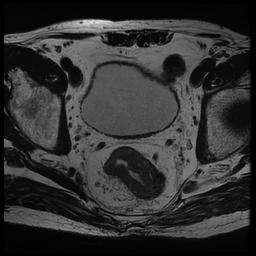
\includegraphics[width=.3\textwidth]{images/T2AX_Alta_8.png}\hfill
    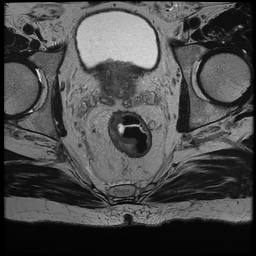
\includegraphics[width=.3\textwidth]{images/T2AX_BO11_5.png}\hfill
    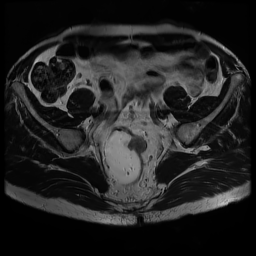
\includegraphics[width=.3\textwidth]{images/T2AX_BO1_9.png}
    
    \caption{T2 weighted axial colorectal cancer MR images. From original dataset}
    \label{trittico}
    
    \end{figure}

In order to get information about diagnosis, therapeutic effect evaluation on colorectal cancer, radiomic analysis can be performed on radiological images through the application of dedicated radiomic algorithms based on segmentation and features extraction. By segmentation we mean the determination of the regions of interest (ROI) in images that are going to be analyzed. In clinical routines, it is carried with manual or semi-manual techniques by radiologists, but this process is time-consuming, highly operator-dependent and subject to operator expertise \cite{jovana, tesicoppola,Trebeschi2017}. Lately, several deep learning techniques in the medical field have been developed exploiting Convolutional Neural Networks (CNN) for medical images segmentation \cite{Trebeschi2017, jovana, tesicoppola}. 

As regard the colorectal cancer segmentation on T2-weighted magnetic resonance, one of the most important study of Trebeschi et al. \cite{Trebeschi2017}, shows how the deep learning approach can perform accurate localization and segmentation of rectal cancer in MR imaging in the majority of patients despite the diffuclt in segmenting a quite important Field-of-View (FOV) as in colorecatal MR images. In Fact, it has been shown how the network performances can vary training the same model with different image annotations or 'labels', taken from different experts, resulting in different Dice-Coefficient (DSC) scores, DSC=0.68 for "reader 1" and DSC=0.70 for "reader 2" respectively. Moreover, not only the labels but also the kind of image, that is to say the kind of tumor can affect the performances of the Networks as resulted in the study of Jovana Panic at al.\cite{panic}, where including cases of mucinous characterized by bright tumoral areas compared to adenocarcinoma, the Dice-Coefficient results in a lower value, in particular DSC=0.58. An overall study about the comparison of different models, in particular different U-Net architectures, for the segmentation of colorectal cancer on T2-weighted magnetic resonance has been carried by Yi-Jie Huang at al.\cite{Huang_2020}, resulting in a Dice-Coefficient score range between 0.52 and 0.75.\\
As regard Radiomic features we meant the features coming from radiographic medical images, which can potentially uncover disease characteristics that fail to be appreciated by the naked eye\cite{wiki:Radiomics}.  
\\
\begin{figure}[htp]
	\centering
	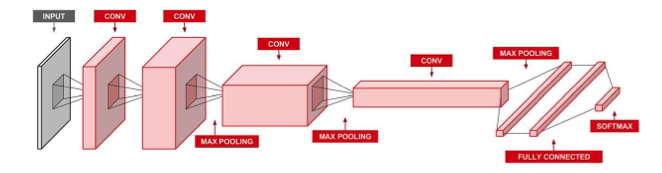
\includegraphics[width=0.9\linewidth]{images/TrebeschiCNN.png}
	\caption{Example of CNN. From \cite{Trebeschi2017} }
\end{figure}

Radiomics features can be divides in different class: shape-size based-features, Haralick's features (Energy, Entropy, Contrast etc...), image voxel descriptors features called GLCM(gray-level co.occurence matrix) and so on. In order to get useful information about the tumor, after segmentation, different approaches have been exploited in literature. For example, in a study of Soomoro at al. \cite{Haraliks}, on T2-weighted magnetic resonance images of colorectal cancer, Haralick's features have been exploited to study the cancer evolution after a segmentation and calssification of tumors depending on the stage malignacy. Another approach consists in clustering all the extracted features after segmentation, in order to get the most relevant ones, as carried in a study of Parmar et al.\cite{featurescluster}.\\
The aim of this project is to implement an automated pipeline based on segmentation and features extraction. As regard the former CNN such as U-Net has been trained from original T2-weighted magnetic resonance images of colorectal cancer dataset, coming from Sant'Orsola Hospital in Bologna, in order to obtain a model to segmented colorectal tumor. As regard the latter, all the possibile features have been extracted for all the patients' examinations and after a reduction analysis the most important ones have been used, integrating clinical data, to predict the response of the patient to the neo-adjuvant chemo-radiotherapy on colorectal cancer. (provvisorio)


\chapter{Segmentation}


\section{Medical Images}


\paragraph{DICOM}
\paragraph{ROI}

\section{Methods review}

\subsection{Thresholding}
\subsection{Region growing}
\subsection{Clustering}
\subsection{U-Net}


\chapter{Radiomics}


\section{First Order Features}
\section{Second Order Features}



\chapter{Pipeline}


\section{Description}

\section{Implementation}

\subsection{Pre-processing}
\subsection{Training}
\subsection{Segmentation outcomes}
\subsection{Features Extraction}
\subsection{Predictions}


\chapter{Results}


\section{Dataset}

\section{Segmentation}

\subsection{Training}
\subsection{Segmentation outcomes}

\section{Features Extraction}

\section{Predictions}


\chapter{Conclusions}


\clearpage

\bibliographystyle{unsrturl}
\bibliography{bibliography}



\end{document}